\documentclass[11pt]{article}
\usepackage{mathtools}
\usepackage{mdframed}
\usepackage{fullpage}
\usepackage{amsfonts}
\usepackage{tikz}
\usepackage{fancyhdr}
\usepackage{lastpage}
\usepackage{listings}
\usepackage{color}
\definecolor{lightgray}{rgb}{.9,.9,.9}
\definecolor{darkgray}{rgb}{.4,.4,.4}
\definecolor{purple}{rgb}{0.65, 0.12, 0.82}
\lstdefinelanguage{JavaScript}{
  keywords={break, case, catch, continue, debugger, default, delete, do, else, false, finally, for, function, if, in, instanceof, new, null, return, switch, this, throw, true, try, typeof, var, void, while, with},
  morecomment=[l]{//},
  morecomment=[s]{/*}{*/},
  morestring=[b]',
  morestring=[b]",
  ndkeywords={class, export, boolean, throw, implements, import, this},
  keywordstyle=\color{blue}\bfseries,
  ndkeywordstyle=\color{darkgray}\bfseries,
  identifierstyle=\color{black},
  commentstyle=\color{purple}\ttfamily,
  stringstyle=\color{red}\ttfamily,
  sensitive=true
}

\lstset{
   language=JavaScript,
   backgroundcolor=\color{lightgray},
   extendedchars=true,
   basicstyle=\footnotesize\ttfamily,
   showstringspaces=false,
   showspaces=false,
   numbers=left,
   numberstyle=\footnotesize,
   numbersep=9pt,
   tabsize=2,
   breaklines=true,
   showtabs=false,
   captionpos=b
}
\usetikzlibrary{automata, positioning}


%edit this for each class
\newcommand\name{John Collin Vincent}
\newcommand\classname{Com S 311}
\newcommand\assignment{Homework 6}


\newcounter{excounter}
\setcounter{excounter}{1}
\newcommand\ques[2]{\vskip 1em  \noindent\textbf{\arabic{excounter}\addtocounter{excounter}{1}.} \emph{#1} \noindent#2}
\newenvironment{question}{\ques{}\begin{quote}}{\end{quote}}
\newenvironment{subquestion}[1]{#1) \begin{quote}}{\end{quote}}

\pagestyle{fancy}
\rfoot{\name, page \thepage/\pageref{LastPage}}
\cfoot{}
\rhead{}
\lhead{}
\renewcommand{\headrulewidth}{0pt}
\renewcommand{\footrulewidth}{0pt}
\DeclarePairedDelimiter\ceil{\lceil}{\rceil}
\DeclarePairedDelimiter\floor{\lfloor}{\rfloor}


\begin{document}


  {\bf \classname \hspace{1cm} \assignment\hfill \name}
  \vskip 2em


  \begin{question}
    \begin{subquestion}{a}
      \centering
      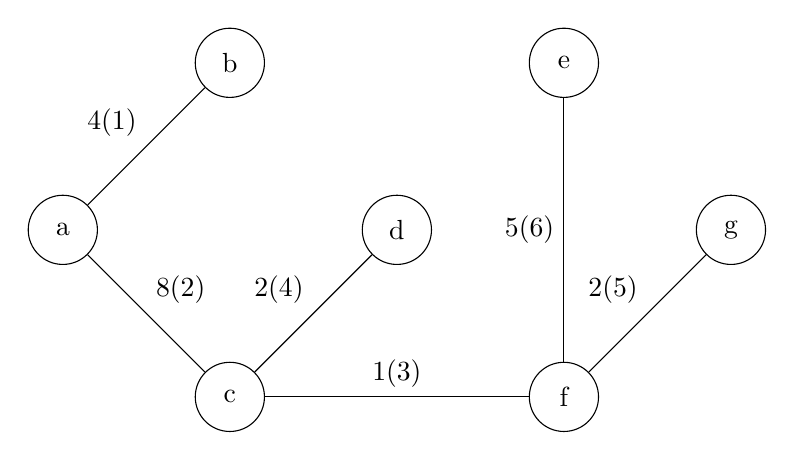
\begin{tikzpicture}[node distance=3cm,bend angle=45,auto]
        \node[state] (n1) {a};
        \node[state] (n2) [above right of = n1] {b};
        \node[state] (n3) [below right of = n1] {c};
        \node[state] (n4) [below right of = n2] {d};
        \node[state] (n5) [above right of = n4] {e};
        \node[state] (n6) [below right of = n4] {f};
        \node[state] (n7) [above right of = n6] {g};

        \path[-] (n1)
          edge node {$4(1)$} (n2)
          edge node {$8(2)$} (n3);

        \path[-] (n3)
          edge node {$2(4)$} (n4)
          edge node {$1(3)$} (n6);

        \path[-] (n6)
          edge node {$2(5)$} (n7)
          edge node {$5(6)$} (n5);
      \end{tikzpicture}
    \end{subquestion}

    \begin{subquestion}{b}
      \centering
      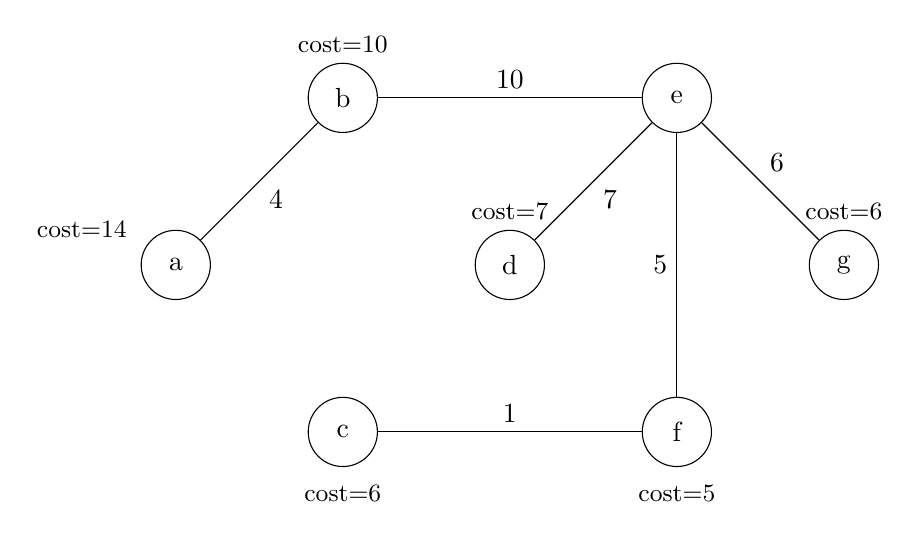
\begin{tikzpicture}[node distance=3cm,bend angle=45,auto]
        \node[state, label={[left = .5cm]\small cost=14}] (n1) {a};
        \node[state, label={[above]\small cost=10}] (n2) [above right of = n1] {b};
        \node[state, label={[below = 1cm]\small cost=6}] (n3) [below right of = n1] {c};
        \node[state, label={[above]\small cost=7}] (n4) [below right of = n2] {d};
        \node[state] (n5) [above right of = n4] {e};
        \node[state,label={[below = 1cm]\small cost=5}] (n6) [below right of = n4] {f};
        \node[state,label={[above]\small cost=6}] (n7) [above right of = n6] {g};

        \path[-] (n3)
          edge node {$1$} (n6);

        \path[-] (n2)
          edge node {$10$} (n5)
          edge node {$4$} (n1);

        \path[-] (n5)
          edge node {$7$} (n4)
          edge node {$6$} (n7);

        \path[-] (n6)
          edge node {$5$} (n5);
      \end{tikzpicture}
    \end{subquestion}
  \end{question}
  \clearpage
  \begin{question}
    Assume there is a graph $G$ such that the graph resulting from running this algorithm $G'$ is
    not a MST of $G$. $G'$ prime cannot have any cycles since if there is a cycle in $G'$ the largest edge in the cycle will be removed before the algrorithm finishes, since it can be removed without leaving any disconnected components. This means that $G'$ is at least a spanning
    tree of $G$. if $G'$ is not a minimum spanning tree that means there must be a edge $e$ in $G'$
    that can be removed and replaced with a path $p$ in $G$ that connects the two components
    connected by $e$, and the sum of the weights in $|p| < |e|$. This can't be the case though
    because if it was $e$ would have been removed from $G'$ before any of the edges in $p$ were visited, since removing $e$ would still keep the components connected through $p$ and
    $e$ must have a weight larger than every edge in $p$. This contradicts $G'$ not being a MST of
    $G$ and proves that this algorithm results in a MST of $G$
  \end{question}

  \begin{question}
    you can follow Kosaraju's algorithm until the first strongly connected component is found, then do a DFS on that first component and if it visits all the nodes in the
    graph that any of the nodes in that SCC will be dominating verticies. This works because Kosaraju's algorithm adds vertices to a stack based on the DFS finish time,
    this ensures that if there is a SCC that can reach all other SCC's then at least on of its vertices will be placed on the top of the stack because even if
    it is selected first all other DFS will finish before on of it vertices finishes. Assume there is a Vertex $V$ that is Dominating that is not in the first SCC $C$
    found by Kosaraju's algorithm. There must be a path from $V$ to $C$ since $V$ is dominating. There cannot be an path from $C$ to $V$
    since that would make a cycle between $C$ and $V$, which would make $V$ part of $C$. If a DFS is run on $C$ then every node in $C$ will finished its DFS and be added to
    the stack, without reaching $V$ and then $V$ will have DFS run on it and be added to the stack contradicting $C$ being the first SCC. If Kosaraju's is started on $V$ then
    it will reach $C$ and every vertex in $C$ will finished its DFS before $V$ does since $C$ was reached durring $V's$ DFS again contradicting $C$ being the first SCC found.
    proving that if there is a dominating vertex in a graph it must be the vertices in the first SCC found by Kosaraju's. Since Kosaraju's algorithm is $O(V+E)$ and then another
    DFS is run with is also $O(V+E)$ so the overall complexity is $O(V+E)$
  \end{question}

  \begin{question}
    the recurrence relation is for the sum of a subset of $A$ where $A = \{a_1,\ldots,a_n\}$, and $\frac{a_1 + a_2 +\ldots+a_n}{2} = j$ is
    \[
      Sum(n,j) =
      \begin{cases}
         Max( \hspace{.2cm}Sum(n-1,j), \hspace{.2cm}a_{n} + Sum(n, j-a_{n}) \hspace{.2cm}) & a_{n} \le j\\
         Sum(n-1, j) & a_{n} > j
      \end{cases}
    \]
    this is correct because it will sum up all the elements it can to get as close as it can to $j$ if the sum function then returns $j$ then we know there
    is a subset of $A$ that will sum up to half of $A's$ sum, if element $a_n$ can fit into $j$ and using it makes the sum closer to $j$ then its used other wise
    it is excluded from the sum, so each possible combination is explored by the end.\\\\
    im leaving my algorithm in JS because it took me forever to figure out and js is super readable anyway. \\ also pushing it down to the next page so the page break doesn't split the
    code.

    \begin{lstlisting}[language=javascript]
      function subSum(A){
        var sum = 0;
        var table = [];
        var min =0;
        var max = 0;
        for ( i = 0; i < A.length; i++){
          sum += A[i];
          table[i] = [];
          if(A[i] < 0){
            min += A[i];
          } else{
            max += A[i];
          }
        }
        if(min > 0){
          min = 0; 
        }
        if(max < 0){
          max = 0;
        }

        table[A.length] = [];
        sum /= 2;
        console.log(sum, min, max);

        for(i = 0; i <= A.length; i++){
          for(j = min; j<= max; j++){
            if(i == 0){
              table[i][j-min] = (j == 0);
            } else if(table[i-1][j - min]){
              table[i][j-min] = true;
            } else{
              table[i][j-min] = A[i-1] == j || (j-A[i-1] >= min && j-A[i-1] <= max && table[i-1][j-A[i-1] - min] == true);
            }
          }
          console.log(table[i]);
        }
        return table[A.length][sum - min] == true;
      }
    \end{lstlisting}
    The time bound for my algorithm is $O(n*D)$ where $D$ is the difference between the max sum and min sum. This is because the first loop runs through the set $A$
    which is size $n$ and then the next loop runs from the min sum to the max sum for each element in $A$.
  \end{question}
  \clearpage
  \begin{question}
    \begin{subquestion}{a}
      \begin{lstlisting}[language=javascript]
        function getDiamonds(x, y){
          r = grid[x+1][y];
          d = grid[x][y+1];
          di = grid[x+1][y+1] + 1;

          if( di >= d && di >= r && M < x && N < y ){
            return getDiamonds(x+1, y+1) - 4 grid[x][y];
          }
          if( r >= d && M < x ){
            return getDiamonds(x+1, y) - 2 + grid[x][y];
          }
          if(N < y){
            return getDiamonds(x, y+1) -2 + grid[x][y];
          }
          return grid[x][y];
        }
      \end{lstlisting}
      if there are no diamonds around the current location the algorithm will go diaginal because this will reduce movement cost, but if there is a 10 value diamond two below
      going two down will yield more diamonds
      \center
      \begin{tabular}{|c|c|c|c|c|}
        \hline
        S & 0 & 0 & 0 & 0\\\hline
        0 & 0 & 0 & 0 & 0\\\hline
        10 & 0 & 0 & 0 & E\\\hline
      \end{tabular}\\\vspace{.2cm}
      \raggedright
      the greedy algorithm will go diagonal twice and right twice encuring a cost of 10 will the optimal route will go down twice and right 4 times encuring a cost of 2.
    \end{subquestion}
    \clearpage
    \begin{subquestion}{b}
      \vspace{-.5cm}
      \begin{lstlisting}[language=javascript]
        function getDiamonds(x, y, ex, ey, a){
          var table = [];
          var max = 0;
          for(i = 0; i < ex-x; i++){
            table[i] = [];
            for(j = 0; j < ey-y; j++){
              max = 0;
              if( i == 0 && j == 0){
                table[i][j] = a[i+x][j+y];
              }else{
                if(i > 0 && j > 0){
                  max = table[i-1][j-1] - 3;
                  if( max < table[i-1][j] -2){
                    max = table[i-1][j] - 2;
                  }
                  if( max < table[i][j-1] -2){
                    max = table[i][j-1] - 2;
                  }
                }else if( i > 0){
                  max = table[i-1][j] - 2;
                } else{
                  max = table[i][j-1] - 2;
                }
                table[i][j] = max + a[i+x][j+y];
              }
            }
          }
          return table[ex-x-1][ey-y-1]
        }
      \end{lstlisting}
      leaving the code in js again, the time complexity is $O(M*N)$
      because we only need to loop from the starting poing to the ending point and fill out the matrix;
    \end{subquestion}
  \end{question}

\end{document}
